\documentclass[11pt,a4paper]{report}
\usepackage[textwidth=37em,vmargin=30mm]{geometry}
\usepackage{calc,xunicode,amsmath,amssymb,paralist,enumitem,tabu,booktabs,datetime2,xeCJK,xeCJKfntef,listings}
\usepackage{tocloft,fancyhdr,tcolorbox,xcolor,graphicx,eso-pic,xltxtra,xelatexemoji}

\newcommand{\envyear}[0]{2025}
\newcommand{\envdatestr}[0]{2025-06-28}
\newcommand{\envfinaldir}[0]{webdb/2025/20250628/final}

\usepackage[hidelinks]{hyperref}
\hypersetup{
    colorlinks=false,
    pdfpagemode=FullScreen,
    pdftitle={Web Digest - \envdatestr}
}

\setlength{\cftbeforechapskip}{10pt}
\renewcommand{\cftchapfont}{\rmfamily\bfseries\large\raggedright}
\setlength{\cftbeforesecskip}{2pt}
\renewcommand{\cftsecfont}{\sffamily\small\raggedright}

\setdefaultleftmargin{2em}{2em}{1em}{1em}{1em}{1em}

\usepackage{xeCJK,xeCJKfntef}
\xeCJKsetup{PunctStyle=plain,RubberPunctSkip=false,CJKglue=\strut\hskip 0pt plus 0.1em minus 0.05em,CJKecglue=\strut\hskip 0.22em plus 0.2em}
\XeTeXlinebreaklocale "zh"
\XeTeXlinebreakskip = 0pt


\setmainfont{Brygada 1918}
\setromanfont{Brygada 1918}
\setsansfont{IBM Plex Sans}
\setmonofont{JetBrains Mono NL}
\setCJKmainfont{Noto Serif CJK SC}
\setCJKromanfont{Noto Serif CJK SC}
\setCJKsansfont{Noto Sans CJK SC}
\setCJKmonofont{Noto Sans CJK SC}

\setlength{\parindent}{0pt}
\setlength{\parskip}{8pt}
\linespread{1.15}

\lstset{
	basicstyle=\ttfamily\footnotesize,
	numbersep=5pt,
	backgroundcolor=\color{black!5},
	showspaces=false,
	showstringspaces=false,
	showtabs=false,
	tabsize=2,
	captionpos=b,
	breaklines=true,
	breakatwhitespace=true,
	breakautoindent=true,
	linewidth=\textwidth
}






\newcommand{\coverpic}[2]{
    % argv: itemurl, authorname
    Cover photo by #2~~(\href{#1}{#1})
}
\newcommand{\makeheader}[0]{
    \begin{titlepage}
        % \newgeometry{hmargin=15mm,tmargin=21mm,bmargin=12mm}
        \begin{center}
            
            \rmfamily\scshape
            \fontspec{BaskervilleF}
            \fontspec{Old Standard}
            \fontsize{59pt}{70pt}\selectfont
            WEB\hfill DIGEST
            
            \vfill
            % \vskip 30pt
            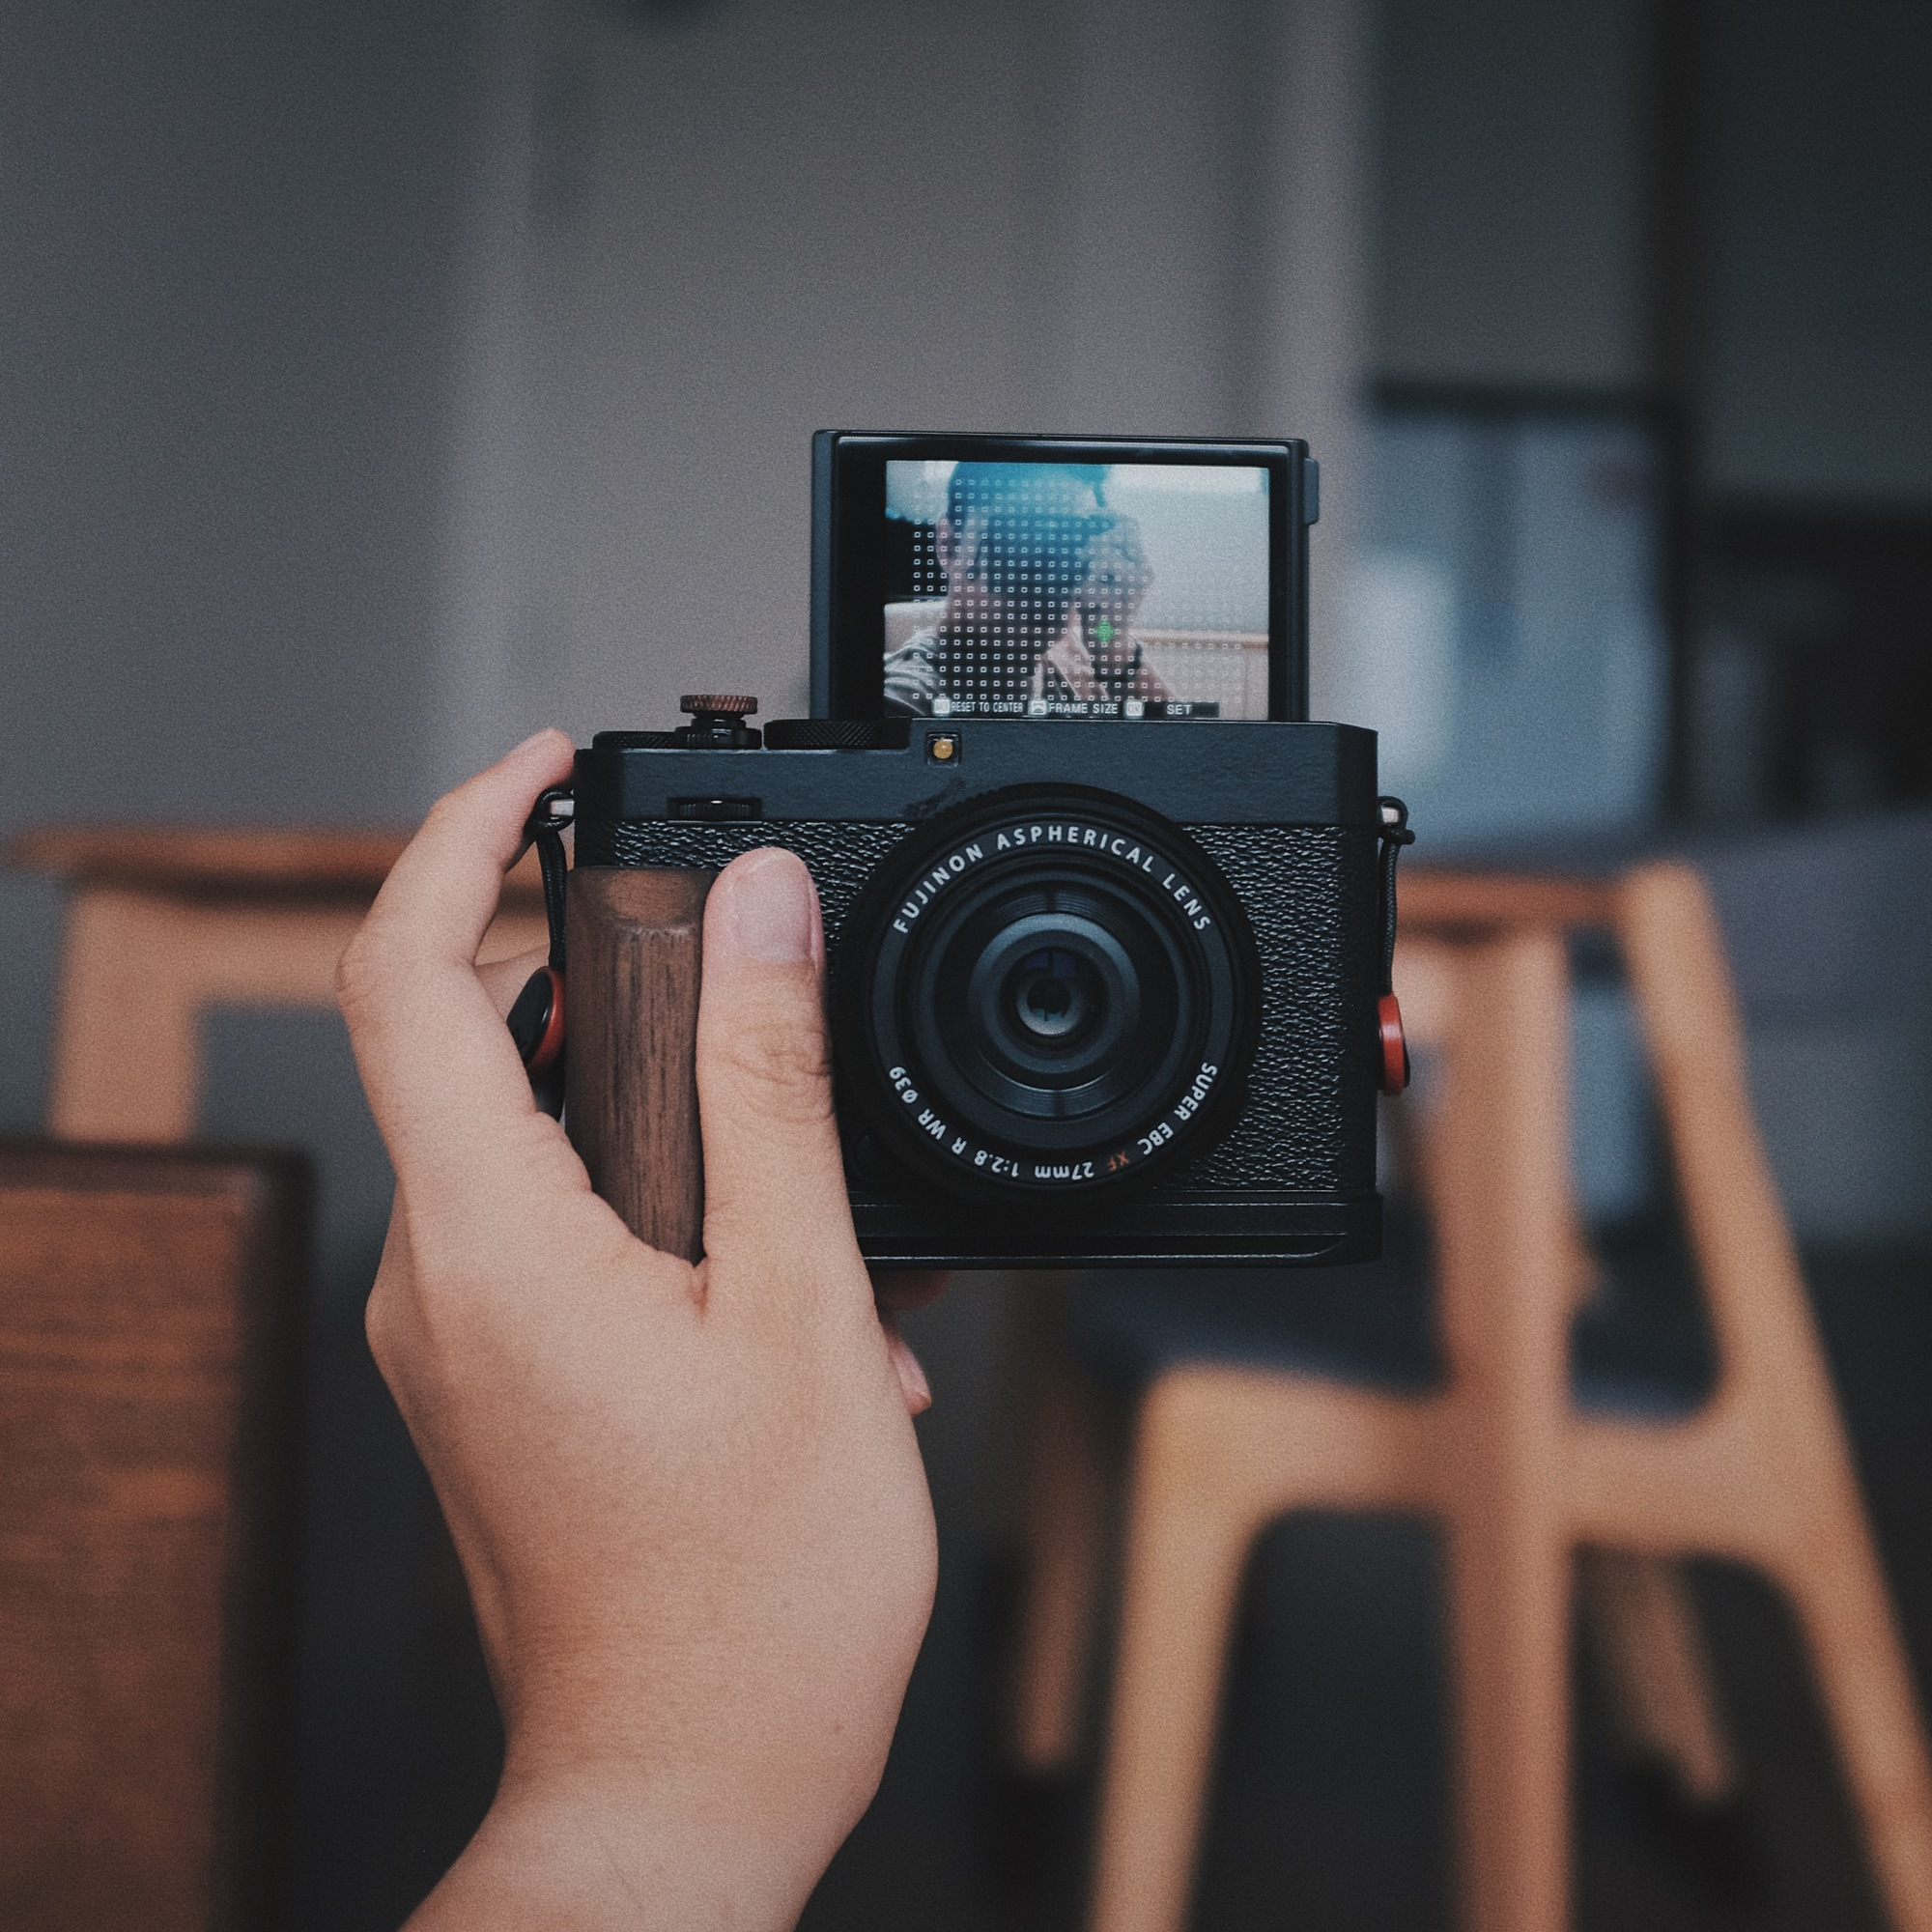
\includegraphics[width=\linewidth]{\envfinaldir/coverpic-prod.jpg}\par
            % \vskip 30pt
            \vfill

            \normalsize\rmfamily\scshape
            \copyright{} The Web Digest Project \hfill\large \envdatestr
        \end{center}
    \end{titlepage}
    % \restoregeometry
}
\newcommand{\simplehref}[1]{%
    \textcolor{blue!80!green}{\href{#1}{#1}}%
}
\renewcommand{\contentsname}{\center\Huge\sffamily\bfseries Contents\par\vskip 20pt}
\newcounter{ipartcounter}
\setcounter{ipartcounter}{0}
\newcommand{\ipart}[1]{
    % \vskip 20pt
    \clearpage
    \stepcounter{ipartcounter}
    \phantomsection
    \addcontentsline{toc}{chapter}{#1}
    % \begin{center}
    %     \Huge
    %     \sffamily\bfseries
    %     #1
    % \end{center}
    % \vskip 20pt plus 7pt
}
\newcounter{ichaptercounter}
\setcounter{ichaptercounter}{0}
\newcommand{\ichapter}[1]{
    % \vskip 20pt
    \clearpage
    \stepcounter{ichaptercounter}
    \phantomsection
    \addcontentsline{toc}{section}{\numberline{\arabic{ichaptercounter}}#1}
    \begin{center}
        \Huge
        \sffamily\bfseries
        #1
    \end{center}
    \vskip 20pt plus 7pt
}
\newcommand{\entrytitlefont}[1]{\subsection*{\raggedright\Large\sffamily\bfseries#1}}
\newcommand{\entryitemGeneric}[2]{
    % argv: title, url
    \parbox{\linewidth}{
        \entrytitlefont{#1}\par\vskip 5pt
        \footnotesize\ttfamily\mdseries
        \simplehref{#2}
    }\vskip 11pt plus 11pt minus 1pt
}
\newcommand{\entryitemGithub}[3]{
    % argv: title, url, desc
    \parbox{\linewidth}{
        \entrytitlefont{#1}\par\vskip 5pt
        \footnotesize\ttfamily\mdseries
        \simplehref{#2}\par\vskip 5pt
        \small\rmfamily\mdseries#3
    }\vskip 11pt plus 11pt minus 1pt
}
\newcommand{\entryitemAp}[3]{
    % argv: title, url, desc
    \parbox{\linewidth}{
        \entrytitlefont{#1}\par\vskip 5pt
        \footnotesize\ttfamily\mdseries
        \simplehref{#2}\par\vskip 5pt
        \small\rmfamily\mdseries#3
    }\vskip 11pt plus 11pt minus 1pt
}
\newcommand{\entryitemHackernews}[3]{
    % argv: title, hnurl, rawurl
    % \parbox{\linewidth}{
    %     \entrytitlefont{#1}\par\vskip 5pt
    %     \footnotesize\ttfamily\mdseries
    %     \simplehref{#3}\par
    %     \textcolor{black!50}{\href{#2}{#2}}
    % }\vskip 11pt plus 11pt minus 1pt
    \begin{minipage}{\linewidth}
            \entrytitlefont{#1}\par\vskip 5pt
            \footnotesize\ttfamily\mdseries
            \simplehref{#3}\par
            \textcolor{black!50}{\href{#2}{#2}}
    \end{minipage}\par\vskip 11pt plus 11pt minus 1pt
}







\begin{document}

\makeheader

\tableofcontents\clearpage




\ipart{Developers}
\ichapter{Hacker News}
\entryitemTwoLinks{US Supreme Court limits federal judges' power to block Trump orders}{https://news.ycombinator.com/item?id=44398710}{https://www.theguardian.com/us-news/2025/jun/27/trump-supreme-court-birthright-citizenship-scotus}

\entryitemTwoLinks{Project Vend: Can Claude run a small shop? (And why does that matter?)}{https://news.ycombinator.com/item?id=44397923}{https://www.anthropic.com/research/project-vend-1}

\entryitemTwoLinks{Weird Expressions in Rust}{https://news.ycombinator.com/item?id=44397367}{https://www.wakunguma.com/blog/rust-weird-expr}

\entryitemTwoLinks{10 Years of Pomological Watercolors}{https://news.ycombinator.com/item?id=44397168}{https://parkerhiggins.net/2025/04/10-years-of-pomological-watercolors/}

\entryitemTwoLinks{Qwen VLo: From "Understanding" the World to "Depicting" It}{https://news.ycombinator.com/item?id=44397124}{https://qwenlm.github.io/blog/qwen-vlo/}

\entryitemTwoLinks{Show HN: I'm an airline pilot – I built interactive graphs/globes of my flights}{https://news.ycombinator.com/item?id=44396518}{https://jameshard.ing/pilot}

\entryitemTwoLinks{The Effect of Noise on Sleep}{https://news.ycombinator.com/item?id=44396487}{https://www.empirical.health/blog/effect-of-noise-on-sleep/}

\entryitemTwoLinks{Copilot Chat in VS Code is now open source}{https://news.ycombinator.com/item?id=44395782}{https://github.com/microsoft/vscode-copilot-chat}

\entryitemTwoLinks{Show HN: Zenta – Mindfulness for Terminal Users}{https://news.ycombinator.com/item?id=44394929}{https://github.com/e6a5/zenta}

\entryitemTwoLinks{Show HN: Sink – Sync any directory with any device on your local network}{https://news.ycombinator.com/item?id=44394051}{https://github.com/sirbread/sink}

\entryitemTwoLinks{Parameterized types in C using the new tag compatibility rule}{https://news.ycombinator.com/item?id=44393942}{https://nullprogram.com/blog/2025/06/26/}

\entryitemTwoLinks{XSLT – Native, zero-config build system for the Web}{https://news.ycombinator.com/item?id=44393817}{https://github.com/pacocoursey/xslt}

\entryitemTwoLinks{Denmark to tackle deepfakes by giving people copyright to their own features}{https://news.ycombinator.com/item?id=44393749}{https://www.theguardian.com/technology/2025/jun/27/deepfakes-denmark-copyright-law-artificial-intelligence}

\entryitemTwoLinks{Biomolecular shifts occur in our 40s and 60s (2024)}{https://news.ycombinator.com/item?id=44393547}{https://med.stanford.edu/news/all-news/2024/08/massive-biomolecular-shifts-occur-in-our-40s-and-60s--stanford-m.html}

\entryitemTwoLinks{Ask HN: Is anyone else just done with the industry?}{https://news.ycombinator.com/item?id=44393304}{https://news.ycombinator.com/item?id=44393304}

\entryitemTwoLinks{A.I. Is Homogenizing Our Thoughts}{https://news.ycombinator.com/item?id=44391247}{https://www.newyorker.com/culture/infinite-scroll/ai-is-homogenizing-our-thoughts}

\entryitemTwoLinks{Kea 3.0, our first LTS version}{https://news.ycombinator.com/item?id=44390962}{https://www.isc.org/blogs/kea-3-0/}

\entryitemTwoLinks{Starcloud can't put a data centre in space at \$8.2M in one Starship}{https://news.ycombinator.com/item?id=44390781}{https://angadh.com/space-data-centers-1}

\entryitemTwoLinks{Matrix v1.15}{https://news.ycombinator.com/item?id=44390740}{https://matrix.org/blog/2025/06/26/matrix-v1.15-release/}

\entryitemTwoLinks{AI Is Dehumanization Technology}{https://news.ycombinator.com/item?id=44390576}{https://thedabbler.patatas.ca/pages/ai-is-dehumanization-technology.html}


\ipart{Developers~~~~(zh-Hans)}
\ichapter{Solidot}
\entryitemGeneric{\hskip 0pt{}笑声也会感染倭黑猩猩}{https://www.solidot.org/story?sid=81669}

\entryitemGeneric{\hskip 0pt{}数字主权始于桌面:欧洲 Linux 桌面时代有望到来}{https://www.solidot.org/story?sid=81668}

\entryitemGeneric{\hskip 0pt{}AMD 成为 Debian 开发者大会的白金赞助商}{https://www.solidot.org/story?sid=81667}

\entryitemGeneric{\hskip 0pt{}丹麦以赋权公民的方式打击深度伪造}{https://www.solidot.org/story?sid=81666}

\entryitemGeneric{\hskip 0pt{}当美国人遇到新闻付费墙很少有人愿意付费}{https://www.solidot.org/story?sid=81665}

\entryitemGeneric{\hskip 0pt{}研究发现大模型用户理解能力较弱}{https://www.solidot.org/story?sid=81664}

\entryitemGeneric{\hskip 0pt{}微软正将杀毒软件移出 Windows 内核}{https://www.solidot.org/story?sid=81663}

\entryitemGeneric{\hskip 0pt{}Google DeepMind 发布 AlphaGenome}{https://www.solidot.org/story?sid=81662}

\entryitemGeneric{\hskip 0pt{}美国计算机科学专业入学人数出现下降趋势}{https://www.solidot.org/story?sid=81661}

\entryitemGeneric{\hskip 0pt{}美国 K-12 教师将 AI 用于备课和评分}{https://www.solidot.org/story?sid=81660}

\entryitemGeneric{\hskip 0pt{}Fairphone 6 发布}{https://www.solidot.org/story?sid=81659}

\entryitemGeneric{\hskip 0pt{}韦伯望远镜可能首次直接获得系外行星影像}{https://www.solidot.org/story?sid=81658}

\entryitemGeneric{\hskip 0pt{}ispace 登月舱登月失败源于高度计}{https://www.solidot.org/story?sid=81657}

\entryitemGeneric{\hskip 0pt{}一次性电子烟毒性大于传统香烟}{https://www.solidot.org/story?sid=81656}

\entryitemGeneric{\hskip 0pt{}法国里昂淘汰微软软件以实现数字主权}{https://www.solidot.org/story?sid=81655}

\entryitemGeneric{\hskip 0pt{}过度捕捞导致鳕鱼体型缩小一半}{https://www.solidot.org/story?sid=81654}

\entryitemGeneric{\hskip 0pt{}Bernie Sanders 认为如果 AI 提高了员工生产力那么应该推行一周四天工作制}{https://www.solidot.org/story?sid=81653}

\entryitemGeneric{\hskip 0pt{}掌机测试发现游戏在 SteamOS 上的性能高于 Windows 11}{https://www.solidot.org/story?sid=81652}

\entryitemGeneric{\hskip 0pt{}Aaron Sorkin 制作《社交网络》续集}{https://www.solidot.org/story?sid=81651}

\entryitemGeneric{\hskip 0pt{}法官裁决 Meta 使用版权书籍训练大模型属于合理使用 }{https://www.solidot.org/story?sid=81650}\ichapter{V2EX}
\entryitemGeneric{\hskip 0pt{}[分享创造] 用 AI(Manus)折腾出一个职场打工人的常用工具}{https://www.v2ex.com/t/1141587}

\entryitemGeneric{\hskip 0pt{}[问与答] 手机号码被中国移动销号怎么办?}{https://www.v2ex.com/t/1141586}

\entryitemGeneric{\hskip 0pt{}[酷工作] [西安]某大厂 React 前端外包岗}{https://www.v2ex.com/t/1141582}

\entryitemGeneric{\hskip 0pt{}[程序员] gemini-cli 问题 ssl 求助}{https://www.v2ex.com/t/1141581}

\entryitemGeneric{\hskip 0pt{}[硬件] 大概率判定联想拯救者笔记本对 SSD 有兼容性问题,掉盘,不识别}{https://www.v2ex.com/t/1141580}

\entryitemGeneric{\hskip 0pt{}[分享创造] 做了个 AI 生成软著申请材料的网站}{https://www.v2ex.com/t/1141579}

\entryitemGeneric{\hskip 0pt{}[生活] 为什么结婚财产分不明白?}{https://www.v2ex.com/t/1141578}

\entryitemGeneric{\hskip 0pt{}[程序员] 前线开发, AI 真实的让我感受到了领导的权力感,张张嘴就能把事情办妥当}{https://www.v2ex.com/t/1141577}

\entryitemGeneric{\hskip 0pt{}[程序员] 关于 AI 时代下程序员未来的思考}{https://www.v2ex.com/t/1141576}

\entryitemGeneric{\hskip 0pt{}[问与答] grok3 这个 think 和 deepsearch 有啥区别?}{https://www.v2ex.com/t/1141575}

\entryitemGeneric{\hskip 0pt{}[宽带症候群] 被电信整破防了,求苏州联通优惠渠道}{https://www.v2ex.com/t/1141573}

\entryitemGeneric{\hskip 0pt{}[VXNA] 申请收录博客: https://www.seedlinginvest.com/}{https://www.v2ex.com/t/1141572}

\entryitemGeneric{\hskip 0pt{}[问与答] 想用监控摄像头对楼下贴条的识别并推送告警有什么好产品或方案?}{https://www.v2ex.com/t/1141571}

\entryitemGeneric{\hskip 0pt{}[问与答] 大家怎么看养老金征税这件事情}{https://www.v2ex.com/t/1141570}

\entryitemGeneric{\hskip 0pt{}[游戏] 推荐个游戏 Neva}{https://www.v2ex.com/t/1141569}

\entryitemGeneric{\hskip 0pt{}[问与答] 淘一个千元内的安卓机,皮糙耐用的,二手和新机都可,买哪个好一些}{https://www.v2ex.com/t/1141566}

\entryitemGeneric{\hskip 0pt{}[问与答] 求 AI 眼镜推荐}{https://www.v2ex.com/t/1141565}

\entryitemGeneric{\hskip 0pt{}[程序员] 失业在家,一行代码没写给儿子做了一款小程序}{https://www.v2ex.com/t/1141564}

\entryitemGeneric{\hskip 0pt{}[上海] 如何在上海实现多子多福?}{https://www.v2ex.com/t/1141563}

\entryitemGeneric{\hskip 0pt{}[问与答] 各位能推荐个安全的家用摄像头吗}{https://www.v2ex.com/t/1141561}

\entryitemGeneric{\hskip 0pt{}[生活] 换个锁芯花了 680....}{https://www.v2ex.com/t/1141559}

\entryitemGeneric{\hskip 0pt{}[分享发现] 今天这趟滴滴是我坐过最舒服的一次~}{https://www.v2ex.com/t/1141557}

\entryitemGeneric{\hskip 0pt{}[推广] 「会动的浮世绘展 FUKUOKA」将于 2025 年 6 月 28 日起在福冈 JR 博多城举行。曾在东京、名古屋、米兰吸引超 25 万人次的沉浸式展览}{https://www.v2ex.com/t/1141554}

\entryitemGeneric{\hskip 0pt{}[iDev] 用 cursor 写了一个支持,提交 ips 和 dSYMs 的工具,挺漂亮的,有用的话,你们拿去开箱用就行}{https://www.v2ex.com/t/1141553}

\entryitemGeneric{\hskip 0pt{}[宽带症候群] 江苏反诈老毛病, 境外站点可以走代理用国外 dns, cn 域名的怎么办}{https://www.v2ex.com/t/1141552}

\entryitemGeneric{\hskip 0pt{}[程序员] 征集技术反诈的方案}{https://www.v2ex.com/t/1141550}

\entryitemGeneric{\hskip 0pt{}[PayPal] paypal 海外账号打款给支付宝,国内要交税啥的操作吗}{https://www.v2ex.com/t/1141549}

\entryitemGeneric{\hskip 0pt{}[问与答] 京东外卖(闪送)骑手这么拽的吗}{https://www.v2ex.com/t/1141548}

\entryitemGeneric{\hskip 0pt{}[生活] 如果你有钱了 想回农村躺平 你想种什么农作物}{https://www.v2ex.com/t/1141547}

\entryitemGeneric{\hskip 0pt{}[分享发现] 淘宝 APP 闪购页面中部 Banner``今日必得 18.8 红包''点进去后红包使用页面卡顿甚至闪退}{https://www.v2ex.com/t/1141546}

\entryitemGeneric{\hskip 0pt{}[分享创造] 做了一个在线将多行文本转换成单行的在线工具, 欢迎体验}{https://www.v2ex.com/t/1141545}

\entryitemGeneric{\hskip 0pt{}[问与答] pdf to epub 在线转换哪个网站能处理好换行?}{https://www.v2ex.com/t/1141544}

\entryitemGeneric{\hskip 0pt{}[职场话题] 职场小登今天气晕了😡}{https://www.v2ex.com/t/1141542}

\entryitemGeneric{\hskip 0pt{}[分享创造] v 站帖子屏蔽器}{https://www.v2ex.com/t/1141541}

\entryitemGeneric{\hskip 0pt{}[路由器] 网络小白求助,电信 ipoe 连接的电视盒子该如何升级?}{https://www.v2ex.com/t/1141540}

\entryitemGeneric{\hskip 0pt{}[问与答] 关于 RAG 调优的能在工业级应用中落地的方法有课程推荐么?}{https://www.v2ex.com/t/1141539}

\entryitemGeneric{\hskip 0pt{}[Apple] macOS 限免剪贴板 App}{https://www.v2ex.com/t/1141538}

\entryitemGeneric{\hskip 0pt{}[macOS] macOS 上有什么好的安卓模拟器吗?想要运行蛋仔派对}{https://www.v2ex.com/t/1141537}

\entryitemGeneric{\hskip 0pt{}[程序员] 大家接码的手机号都从哪来的的}{https://www.v2ex.com/t/1141536}

\entryitemGeneric{\hskip 0pt{}[分享创造] 我又又有来开源 Vibe 产品了 - 这次是 🤖 Vibe PR Reviewer: 一个 Github PR 审阅机器人}{https://www.v2ex.com/t/1141535}

\entryitemGeneric{\hskip 0pt{}[酷工作] 北京 WLB 公司招聘}{https://www.v2ex.com/t/1141534}

\entryitemGeneric{\hskip 0pt{}[小米] 键盘打工人: 这几块板子的技术含量比其他家全车的空力都高}{https://www.v2ex.com/t/1141531}

\entryitemGeneric{\hskip 0pt{}[程序员] gemini-cli 使用谷歌账户登录不上}{https://www.v2ex.com/t/1141529}

\entryitemGeneric{\hskip 0pt{}[macOS] Raycast 启动器出 windows beta 版本了!}{https://www.v2ex.com/t/1141528}

\entryitemGeneric{\hskip 0pt{}[分享创造] Ai 对于小项目式是颠覆式的。完全不会前端,使用 cursor 上架了简单的 tab 删除插件}{https://www.v2ex.com/t/1141527}

\entryitemGeneric{\hskip 0pt{}[Apple] 请问 iOS 端有管理电影票的 app 么?}{https://www.v2ex.com/t/1141526}

\entryitemGeneric{\hskip 0pt{}[问与答] 如果你看到一篇好文章,但是你当前又要去忙其它事了,你会怎么办?}{https://www.v2ex.com/t/1141525}

\entryitemGeneric{\hskip 0pt{}[职场话题] 以前我一直以为只有女人不能闲着,闲着就容易会找事(例如: 全职妈妈,有大概率就会说老哥陪她的时间少),现在看来男人也一样}{https://www.v2ex.com/t/1141524}

\entryitemGeneric{\hskip 0pt{}[汽车] 小米汽车能被模仿吗?有护城河吗?}{https://www.v2ex.com/t/1141523}

\entryitemGeneric{\hskip 0pt{}[投资] 周末分享一下最近 1 个月在欧易的操作,大家乐一乐}{https://www.v2ex.com/t/1141522}


\ipart{Generic News}







\clearpage
\leavevmode\vfill
\footnotesize

Copyright \copyright{} 2023-2025 Neruthes and other contributors.

This document is published with CC BY-NC-ND 4.0 license.

The entries listed in this newsletter may be copyrighted by their respective creators.

This newsletter is generated by the Web Digest project.

The newsletters are also delivered via Telegram channel \CJKunderline{\href{https://t.me/webdigestchannel}{https://t.me/webdigestchannel}}.\\
RSS feed is available at \CJKunderline{\href{https://webdigest.pages.dev/rss.xml}{https://webdigest.pages.dev/rss.xml}}.

This newsletter is available in PDF at
\CJKunderline{\href{https://webdigest.pages.dev/}{https://webdigest.pages.dev/}}.

The source code being used to generate this newsletter is available at\\
\CJKunderline{\href{https://github.com/neruthes/webdigest}{https://github.com/neruthes/webdigest}}.

This newsletter is also available in
\CJKunderline{\href{http://webdigest.pages.dev/readhtml/\envyear/WebDigest-20250628.html}{HTML}} and
\CJKunderline{\href{https://github.com/neruthes/webdigest/blob/master/markdown/\envyear/WebDigest-20250628.md}{Markdown}}.


\coverpic{https://unsplash.com/photos/a-person-admiring-a-mountain-vista-VeGrU1SIRaM}{Diogo Ferrer}


\end{document}
